\section{RANSAC with Ellipse I (18)}

In this exercise, you are tasked to detect an ellipse based on given dataset using RANSAC.
\begin{figure}[H]
    \centering
    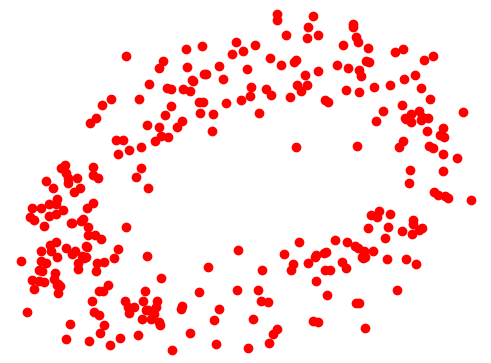
\includegraphics[width=0.65\textwidth]{img/ellipse.png}
    \caption{A Plot of Randomly Selected Dataset}
    \label{fig:p3c1}
\end{figure}
The goal is to estimate the parameters $\mathbf{Q}$ and $\mathbf{b}$ by fitting the sensor data to an ellipse. 
An ellipse can be described by the quadratic equation: 
\begin{equation*}
(\mathbf{p}-\mathbf{b})^\top\mathbf{Q}(\mathbf{p}-\mathbf{b})=1
\end{equation*}
or
\begin{equation*}
    Ax^2+2Bxy+Cy^2-2Dx-2Ey+1=0
\end{equation*}
where:
\begin{itemize}
\item $\mathbf{Q}=\mathbf{Q}^\top\in\mathbb{R}^{2\times2}$ is a unique symmetric positive definite matrix of coefficients. [If $\mathbf{Q}$ is not positive definite, you may have a hyperbola instead.]
\end{itemize}
Note that the coefficients ($A$,$B$,$C$,$D$,and $E$) are also unique.
The conversion from the polynomial coeffcients to the quadratic form can be expressed as follows:
\begin{equation*}
    \begin{aligned}
        \mathbf{Q}&=\alpha\begin{bmatrix}
        A & B\\ B & C
    \end{bmatrix}\\
    \mathbf{Q}\mathbf{b}&=\alpha\begin{bmatrix}
        D\\E
    \end{bmatrix}\\
    \alpha&=\frac{1}{\begin{bmatrix}
        D & E
    \end{bmatrix}\begin{bmatrix}
        A & B \\ B & C
    \end{bmatrix}^{-1}\begin{bmatrix}
        D \\ E
    \end{bmatrix}-1}
    \end{aligned}
\end{equation*}

\begin{enumerate}[a.)]  
\item Determine the minimum number of points to uniquely determined ellipse's parameters as well as derive a method to construct an ellipse with the parameters ($A$,$B$,$C$,$D$, and $E$) based on those points. $\mathbf{p}_i=(x_i,y_i)$ denote the $i^\text{th}$ data point. You must explain your rationale to receive credits. [10 pts]

\textbf{Answer}:

The general form of an ellipse is:
\begin{equation*}
    Ax^2+2Bxy+Cy^2-2Dx-2Ey+1=0
\end{equation*}
From this equation, it is evident that with five unknowns, five points are needed to uniquely determine an ellipse's parameters.
Each point is written as:
\[
p_i = (x_i, y_i)
\]
Substituting \(x = x_i\) and \(y = y_i\) for \(i = 1, 2, 3, 4, 5\) into the ellipse equation.
This results in a system of five linear equations:
\[
\begin{cases}
A x_1^2 + 2B x_1 y_1 + C y_1^2 - 2D x_1 - 2E y_1 + 1 = 0 \\
A x_2^2 + 2B x_2 y_2 + C y_2^2 - 2D x_2 - 2E y_2 + 1 = 0 \\
A x_3^2 + 2B x_3 y_3 + C y_3^2 - 2D x_3 - 2E y_3 + 1 = 0 \\
A x_4^2 + 2B x_4 y_4 + C y_4^2 - 2D x_4 - 2E y_4 + 1 = 0 \\
A x_5^2 + 2B x_5 y_5 + C y_5^2 - 2D x_5 - 2E y_5 + 1 = 0 \\
\end{cases}
\]
Rewriting the above system of linear equations:
\[
\begin{bmatrix}
x_1^2 & 2x_1 y_1 & y_1^2 & -2x_1 & -2y_1 \\
x_2^2 & 2x_2 y_2 & y_2^2 & -2x_2 & -2y_2 \\
x_3^2 & 2x_3 y_3 & y_3^2 & -2x_3 & -2y_3 \\
x_4^2 & 2x_4 y_4 & y_4^2 & -2x_4 & -2y_4 \\
x_5^2 & 2x_5 y_5 & y_5^2 & -2x_5 & -2y_5 \\
\end{bmatrix} \cdot
\begin{bmatrix}
A \\ B \\ C \\ D \\ E
\end{bmatrix}
=
\begin{bmatrix}
-1 \\ -1 \\ -1 \\ -1 \\ -1
\end{bmatrix}
\]
Solving:
\[
\begin{bmatrix}
A \\ B \\ C \\ D \\ E
\end{bmatrix}
=
\begin{bmatrix}
x_1^2 & 2x_1 y_1 & y_1^2 & -2x_1 & -2y_1 \\
x_2^2 & 2x_2 y_2 & y_2^2 & -2x_2 & -2y_2 \\
x_3^2 & 2x_3 y_3 & y_3^2 & -2x_3 & -2y_3 \\
x_4^2 & 2x_4 y_4 & y_4^2 & -2x_4 & -2y_4 \\
x_5^2 & 2x_5 y_5 & y_5^2 & -2x_5 & -2y_5 \\
\end{bmatrix}^{-1} \cdot
\begin{bmatrix}
-1 \\ -1 \\ -1 \\ -1 \\ -1
\end{bmatrix}
\]

\item 
Fit an ellipse with the following datasets and compute for $\mathbf{Q}$, $\mathbf{b}$, $A$, $B$, $C$, $D$ and $E$.

\begin{equation*}
    (2.92, -6.01), \quad (3.40, -7.20), \quad (4.99, -7.84), \quad (5.48, -7.04), \quad (4.20, -5.91)
\end{equation*}

 You don't have code for this part, but you still have to do it with Python in the next part. [8 pts.]

\textbf{Answer}:
Plugging in the points given above into the matrix, we can obtain: \\

\[
\begin{bmatrix}
(2.92)^2 & 2(2.92) (-6.01) & (-6.01)^2 & -2(2.92) & -2(-6.01) \\
(3.40)^2 & 2(3.40) (-7.20) & (-7.20)^2 & -2(3.40) & -2(-7.20) \\
(4.99)^2 & 2(4.99) (-7.84) & (-7.84)^2 & -2(4.99) & -2(-7.84) \\
(5.48)^2 & 2(5.48) (-7.04) & (-7.04)^2 & -2(5.48) & -2(-7.04) \\
(4.20)^2 & 2(4.20) (-5.91) & (-5.91)^2 & -2(4.20) & -2(-5.91) \\
\end{bmatrix} \cdot
\begin{bmatrix}
A \\ B \\ C \\ D \\ E
\end{bmatrix}
=
\begin{bmatrix}
-1 \\ -1 \\ -1 \\ -1 \\ -1
\end{bmatrix}
\]

\[
\begin{bmatrix}
8.5264 & -35.0984 & 36.1201 & -5.84 & 12.02 \\
11.56 & -48.96 & 51.84 & -6.80 & 14.40 \\
24.9001 & -78.2432 & 61.4656 & -9.98 & 15.68 \\
30.0304 & -77.1584 & 49.5616 & -10.96 & 14.08 \\
17.64 & -49.644 & 34.9281 & -8.40 & 11.82 \\
\end{bmatrix} \cdot
\begin{bmatrix}
A \\ B \\ C \\ D \\ E
\end{bmatrix}
=
\begin{bmatrix}
-1 \\ -1 \\ -1 \\ -1 \\ -1
\end{bmatrix}
\]
Solving the system of equations yields:
\[
    \begin{bmatrix}
        A \\
        B \\
        C \\
        D \\
        E
        \end{bmatrix} = \begin{bmatrix}
        0.01806 \\
        0.01207 \\
        0.03015 \\
        -0.00625 \\
        -0.15441
        \end{bmatrix}
\]
Finding \textbf{Q} and \textbf{b}
\[
    \alpha = \frac{1}{\begin{bmatrix} D & E \end{bmatrix} \begin{bmatrix} A & B \\ B & C \end{bmatrix}^{-1} \begin{bmatrix} D \\ E \end{bmatrix} - 1}
\]
\[
    \alpha = \frac{1}{\begin{bmatrix} (-0.00625) & (-0.15441) \end{bmatrix} \begin{bmatrix} (0.01806) & (0.01207) \\ (0.01207) & (0.03015) \end{bmatrix}^{-1} \begin{bmatrix} (-0.00625) \\ (-0.15441) \end{bmatrix} - 1} = 41.67811288
\]

\[
\mathbf{Q} =\alpha\begin{bmatrix}
    A & B\\ B & C
\end{bmatrix} = 41.67811288
\begin{bmatrix}
    0.01806 & 0.01207 \\
0.01207 & 0.03015
\end{bmatrix} = \begin{bmatrix}
    0.75282437&0.50302811 \\
    0.50302811&1.25673065
    \end{bmatrix}
\]
\[
\mathbf{b} =\alpha \mathbf{Q}^{-1} \begin{bmatrix}
    D\\E
\end{bmatrix} = 41.67811288 \begin{bmatrix}
    0.75282437&0.50302811 \\
    0.50302811&1.25673065
    \end{bmatrix}^{-1}\begin{bmatrix}
    -0.00625 \\
    -0.15441 \end{bmatrix} = \begin{bmatrix}
        4.19868909 \\
        -6.80150371 \end{bmatrix}
\]

\end{enumerate}
